\documentclass[cjk,c,squeeze,shrink,dvipdfmx,12pt]{beamer}
% 以下は決まり文句
\usepackage{bxdpx-beamer}                      % dvipdfmx用の fix
\usepackage{pxjahyper}                         % 日本語で'しおり'
\usepackage{minijs}                            % min10ヤダ
\renewcommand{\kanjifamilydefault}{\gtdefault} % 既定をゴシック体に

\usetheme{KansaiDebian}
\usepackage{amsmath,amssymb,ulem}
\AtBeginSection[]{%
  \begin{frame}<beamer>\frametitle{Agenda}\tableofcontents[currentsection]\end{frame}}

\title[Debian Updates: Buster]{Debian Updates: Buster}
\subtitle[OSC 2019 Kyoto]{〜オープンソースカンファレンス 2019 Kyoto〜}
\author[かわだ]{%
  かわだてつたろう/Tetsutaro KAWADA\\[1em]
  \href{mailto:t3rkwd@debian.or.jp}{t3rkwd@debian.or.jp}
}
\institute[Debian JP Project]{%
  {\footnotesize{%
      Debian JP Project/関西Debian勉強会
    }}
}
\date[2019/08/03]{%
  {\tiny{2019年08月03日@京都リサーチパーク}}
}

\begin{document}
\setbeamercovered{transparent}
\takahashi[80]{ }
{%
  \setbeamertemplate{headline}{}
  \setbeamertemplate{footline}{}
  \begin{frame}
    \maketitle
  \end{frame}
}

\begin{frame}[fragile]
  \frametitle{Disclaimer}
  \begin{itemize}
  \item 疑問、質問、ツッコミ、茶々、\alert{大歓迎}
  \item その場でインタラクティブにどうぞ
  \item ハッシュタグ \alert{\#debianjp} で
  \end{itemize}
\end{frame}

\begin{frame}[fragile]{Agenda}
  \tableofcontents
\end{frame}
%-------------------

\section{Debianとは? Debian JP とは?}
\takahashi[60]{Debianとは?}

\begin{frame}[fragile]{Debian とは?}

  \alert{フリー/オープン}な\alert{ユニバーサル}オペレーティングシステムを
  作成しようとするボランティアベースのプロジェクト。

  \vfill
  \centering
  \begin{tabular}{|c|c|c|}
    \hline
    ディストリ & 企業 & ボランティア \\ \hline
    Fedora & RedHat支援あり & あり  \\ \hline
    RHEL & RedHat & なし  \\ \hline
    CentOS & RedHat支援あり & あり \\ \hline
    \color{red}{Debian}  & \color{red}{なし} & \color{red}{あり} \\ \hline
    Ubuntu  & Canonical & あり \\ \hline
    openSUSE & SUSE支援あり & あり \\ \hline
    SLES & SUSE & なし \\ \hline
  \end{tabular}
  \vfill
\end{frame}


\begin{frame}[fragile]{Debian とは?}

  厳格/厳密なポリシーとガイドラインに沿った開発体制
  \begin{itemize}
  \item Debian 社会契約
  \item Debian フリーソフトウェアガイドライン
    \begin{itemize}
    \item オープンソースの定義の元
    \end{itemize}
  \item Debian Policy
  \end{itemize}

\end{frame}

\begin{frame}[fragile]{Debian とは?}
  \begin{columns}
    \begin{column}{.58\paperwidth}
      \begin{itemize}
      \item
        Ubuntu や Raspbian といったディストリビューションのベースとなっている
      \item
        Debian Derivatives(Debian 派生ディストリビューション)との協力体制の整備
      \end{itemize}
    \end{column}
    \begin{column}{.4\paperwidth}
      \centering
      % https://upload.wikimedia.org/wikipedia/commons/thumb/6/69/DebianFamilyTree1210.svg/500px-DebianFamilyTree1210.svg.png
      % \includegraphics[height=.65\paperheight]{image201908/500px-DebianFamilyTree1210.png}
    \end{column}
  \end{columns}
\end{frame}

\begin{frame}[fragile]{Debian とは?}
 世界規模で開発が行われており、63ヶ国、約1,100名のDebian公式開発者が開発を行
 っている。パッケージメンテナや翻訳などの貢献者も入れるともっと多くの開発者が参加
 していることになる。

 \centering
 % https://wiki.debconf.org/upload/thumb/d/da/Dc17logo.png/800px-Dc17logo.png
 % \includegraphics[width=0.4\linewidth]{image201908/800px-Dc17logo.png}
 % https://wiki.debconf.org/upload/thumb/6/60/DebConf18_Horizontal_Logo.png/800px-DebConf18_Horizontal_Logo.png
 % \includegraphics[width=0.4\linewidth]{image201908/800px-DebConf18_Horizontal_Logo.png}
\end{frame}


\begin{frame}[fragile]{Debian とは?}
  2019年8月の時点で、
  \pause
  \begin{itemize}[<+->]
  \item
    最新版は {\alert{Debian 10}}, Buster
  \item
    提供パッケージ数は{\alert{約59,000}}
  \item
    公式にサポートするCPUアーキテクチャは{\alert{10}}
  \item {\alert{約2年毎}}にリリース
  \item next: Debian 11, Bullseye
  \item コードネームはトイ・ストーリーのキャラクターから
  \end{itemize}
\end{frame}

\begin{frame}[fragile]{Debian とは?: まとめ}
  \pause
  \begin{itemize}[<+->]
  \item Debianはフリー/オープンなOSを作成しようとするボランティアベースのプロジェクト。
  \item 自分たちの考えるフリーという言葉に関する定義、開発目的、パッケージングポリシーを厳格に決めている。
  \item 世界中に1,100人以上の開発者がおり、他のディストリビューションのベースとして採用されている。
  \item 約2年毎にリリースが行われ、多くのパッケージとアーキテクチャをサポートしている。
  \item 上記のような特徴から様々なところで利用されているディストリビューションである。
\end{itemize}
\end{frame}

%------------------
\begin{frame}[fragile]{Debian JP Project とは?\\[-.5em]{\normalsize{\texttt{https://www.debian.or.jp}}}}
  \pause
  \begin{itemize}[<+->]
  \item 日本でのDebianの普及を目的とした任意団体。
  \item %
    Debianの日本語による情報発信、
    ユーザとの情報交換、
    Debian 開発者、
    パッケージメンテナの育成など。
  \end{itemize}
\end{frame}


\begin{frame}
  \frametitle{Debian勉強会とは?%
    \\[-.5em]{\normalsize{\texttt{https://tokyodebian-team.pages.debian.net/}}}%
    \\[-.5em]{\normalsize{\texttt{https://wiki.debian.org/KansaiDebian}}}%
  }
  \pause
  \begin{itemize}[<+->]
  \item
    2005年1月開始, Debian Developer 上川さん発起人
  \item
    東京と関西で月に一回コンスタントに開催しているDebian開発者、
    ユーザによる勉強会。
  \item
    何がしたいのか?
    \begin{itemize}[<+->]
    \item
      MLとIRCで情報交換⇒face-to-faceであう場所がない
    \item
      まとまったドキュメントが出てこない
    \end{itemize}
  \item
    Debian勉強会でやっていること
    \begin{itemize}[<+->]
    \item
      定期的に集まる(場の提供)
    \item
      資料を作成して, 公開(GPL-2+) \\
      {\small \url{https://salsa.debian.org/tokyodebian-team/}}
    \end{itemize}
  \end{itemize}

\end{frame}

%-----------------------
\takahashi[40]{Any Questions?}

\section{Debian Updates: Buster}
\takahashi[60]{Debian Updates: Buster}

{%
  \setbeamertemplate{headline}{}
  \setbeamertemplate{footline}{}
  \begin{frame}
    \centering
    % https://bits.debian.org/images/upcoming-buster.png
    % \includegraphics[scale=1]{image201908/upcoming-buster.png}
  \end{frame}
}

\takahashi[60]{Debian 10 Buster Released!}

\begin{frame}[fragile]{%
    Debian Updates: Buster%
    \\[-.5em]{\normalsize{Release Timetable}}
  }
  \pause
  \begin{itemize}[<+->]
  \item 2014/11/09: Distribution codename announced
  \item 2017/06/17: Stretch is released, and buster becomes testing
  \item 2019/01/12: Transition freeze
  \item 2019/02/12: Soft freeze
  \item 2019/03/12: Full freeze
  \item 2019/07/06: Released!
  \item (2019/09/07: Updated Debian 10.1 released)
  \end{itemize}
\end{frame}

\begin{frame}[fragile]{%
    Debian Updates: Buster%
    \\[-.5em]{\normalsize{Artwork}}
  }
  \begin{itemize}
  \item Alex Makas: futurePrototype
  \end{itemize}
  \begin{center}
    
\includegraphics[width=0.8\hsize]{image201906/futurePrototype-wallpaper-1920x1080.png}
  \end{center}
\end{frame}

\begin{frame}[fragile]{%
    Debian Updates: Buster%
    \\[-.5em]{\normalsize{Architectures}}
  }
  \begin{itemize}
  \item amd64, i386
  \item arm64, armel, armhf
  \item mips64el, mipsel, mips
  \item ppc64el
  \item s390x
  \end{itemize}
\end{frame}

\begin{frame}[fragile]{%
    Debian Updates: Buster%
    \\[-.5em]{\normalsize{Packages \& versions}}
  }
  \begin{itemize}
  \item GNOME 3.30, KDE Plasma 5.14, Cinnamon 3.8, MATE 1.20, Xfce 4.12, LXDE 0.99.2, LXQt 0.14
  \item Linux 4.19 series
  \item Chromium 73.0, Firefox 60.7, Thunderbird 60.7.2
  \item LibreOffice 6.1, GIMP 2.10.8, Inkscape 0.92.4
  \item GNU Compiler Collection 7.4 and 8.3
  \item Perl 5.28, Python 3.7.2, Ruby 2.5.1, PHP 7.3, Golang 1.11, OpenJDK 11, Rustc 1.34
  \item MariaDB 10.3, PostgreSQL 11
  \item Emacs 26.1, Vim 8.1
  \item etc..
  \end{itemize}
\end{frame}

\begin{frame}[fragile]{%
    Debian Updates: Buster%
    \\[-.5em]{\normalsize{New Features (1)}}
  }
  UEFI セキュアブート

  \begin{itemize}
  \item セキュアブートが有効な状態でもインストールと利用ができるようになった
  \item shim-signed, grub-efi-\{amd64,ia32\}-signed, Buster の Linux カーネルパッケージをインストールすれば既存の Debian でも利用可能
  \item DKMS が使用できないなど一部機能の制限あり
  \end{itemize}
\end{frame}

\begin{frame}[fragile]{%
    Debian Updates: Buster%
    \\[-.5em]{\normalsize{New Features (2)}}
  }

  AppArmorの有効化

  \begin{itemize}
  \item 多くのプロファイルは apparmor-profiles-extra をインストールすると利用可能
  \item Linux カーネルパッケージで推奨 (Recommends) 依存設定
  \end{itemize}
\end{frame}

\begin{frame}[fragile]{%
    Debian Updates: Buster%
    \\[-.5em]{\normalsize{New Features (3)}}
  }

  ネットワークフィルタリングの nftables への変更

  \begin{itemize}
  \item iptables コマンドは nftables を使用する iptables-nft がデフォルト
  \item 従来の iptables を使用するコマンドは iptables-legacy として提供
  \item 他のディストリビューションでも同様に変更\\
    e.g. Red Hat Enterprise Linux 8.0
  \end{itemize}
\end{frame}

\begin{frame}[fragile]{%
    Debian Updates: Buster%
    \\[-.5em]{\normalsize{New Features (4)}}
  }

  GNOMEのデフォルトは Wayland

  \begin{itemize}
  \item デフォルトで Wayland を使用
  \item Xorg はデフォルトでインストールされるので切り替えて使用可能
  \end{itemize}
\end{frame}

\begin{frame}[fragile]{%
    Debian Updates: Buster%
    \\[-.5em]{\normalsize{New Features (5)}}
  }

  新規インストールは /usr マージ

\begin{verbatim}
\end{verbatim}
  \begin{center}
    {\Huge{
        \texttt{/bin → /usr/bin}\\
        \texttt{/sbin → /usr/sbin}\\
        \texttt{/lib → /usr/lib}\\
    }}
  \end{center}

  \begin{itemize}
  \item Debian 以外から提供されるソフトウェアを利用している場合は要注意
  \end{itemize}
\end{frame}

\begin{frame}[fragile]{%
    Debian Updates: Buster%
    \\[-.5em]{\normalsize{New Features (6)}}
  }
  \pause
  \begin{itemize}[<+->]
  \item APTへのセキュリティ強化オプションの追加
  \item stable ポイントリリースに対する Unattended-upgrades の挙動
  \item ドイツ語話者用 man ページの飛躍的な改善
  \item Cryptsetup の on-disk LUKS2への変更
  \item CUPS 2.2.10 でのドライバーレス印刷機能
  \item Allwinner A64 ベースのデバイスでの基本機能サポート
  \item などなど
  \end{itemize}
\end{frame}

\begin{frame}[fragile]{%
    Debian Updates: Buster%
    \\[-.5em]{\normalsize{Issues}}
  }
  \pause
  \begin{itemize}[<+->]
  \item リリースノートの翻訳が未完
  \item glibc は Linux カーネル 3.2 以上を必要
  \item Wayland で一部アプリケーションが動作しない\\
    (synaptic, fcitx, アクセシビリティ機能)
  \item phpmyadmin, Redmine, VirtualBox などのパッケージは未収録
  \item Python2.7 は非推奨
  \item More entropy
  \item OpenSSL のデフォルトが TLS 1.2 とセキュリティレベル 2
  \item ブラウザ, レンダリングエンジン, Go 関連のパッケージは制限付きのセキュリティサポート
  \item gnome-disk-utility: LUKS パスワード変更でデータ消失の危険性
  \item などなど
  \end{itemize}
\end{frame}

\begin{frame}[fragile]{%
    Debian Updates: Stretch%
    \\[-.5em]{\normalsize{Debian 9.x: oldstable}}
  }
  \pause
  \begin{itemize}[<+->]
  \item 2017/06/17: Debian 9.0 released
  \item[] :
  \item 2019/01/23: Updated Debian 9.7 released
  \item 2019/02/16: Updated Debian 9.8 released
  \item 2019/04/27: Updated Debian 9.9 released
  \item[] :
  \item \alert{2019/07/06: Becomes oldstable}
  \item[←] oldstable のサポートはここから 1 年
  \item (2019/09/07: Updated Debian 9.10 released)
  \end{itemize}
\end{frame}


\begin{frame}[fragile]{Debian Updates: Debconf}
  \begin{itemize}
  \item 年に一回, Debian 開発者が集って開催するカンファレンス
  \item 今年は
    \alert{2019/07/21 - 07/28: Debconf19: CURITIBA - BRAZIL}
  \end{itemize}
  \begin{center}
    % https://wiki.debian.org/DebConf/19/Artwork?action=AttachFile&do=get&target=800px-Debconf19-horizontal.png
    % \includegraphics[scale=1.0]{image201908/800px-Debconf19-horizontal.png}
  \end{center}
\end{frame}

{%
  \setbeamertemplate{headline}{}
  \setbeamertemplate{footline}{}
  \begin{frame}
    \centering
    % https://salsa.debian.org/debconf-team/public/share/debconf19/raw/master/photos/aigarius/group/debconf19_group_small.jpg
    % 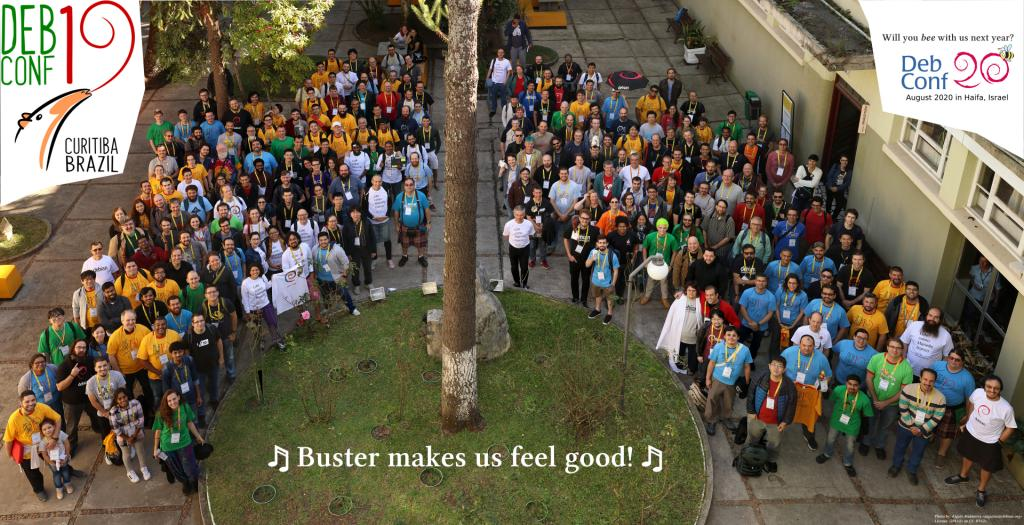
\includegraphics[width=.9\paperwidth]{image201908/debconf19_group_small.jpg}
  \end{frame}
}

\begin{frame}[fragile]{Debian Updates: Debconf}
  \begin{itemize}
  \item 来年は 2020/08/23 - 08/29: Debconf20: Haifa - Israel
    \begin{center}
      % https://wiki.debian.org/DebConf/20/Artwork/LogoProposals?action=AttachFile&do=get&target=dc20-logo-bee.svg
      % \includegraphics[width=.9\paperwidth]{image201908/dc20-logo-bee.png}
    \end{center}
  \end{itemize}
\end{frame}


\takahashi[70]{そんな\\こんなで}

\takahashi[40]{Any Questions?}

\section{日本語によるDebianの情報}
\takahashi[40]{日本語によるDebianの情報}

\begin{frame}[fragile]{日本語によるDebianの情報}
  \begin{itemize}
  \item Debian JP Project \\
    \url{https://www.debian.or.jp}
  \item 東京エリアDebian勉強会\\
    \url{https://tokyodebian.alioth.debian.org}
  \item 関西エリアDebian勉強会 \\
    \url{https://wiki.debian.org/KansaiDebianMeeting}
  \item Twitter \\
    \url{@debian_jp}
  \item slack
    \url{debian-jp.slack.com}
  \end{itemize}
\end{frame}

\begin{frame}
  \frametitle{書籍情報}
  \begin{columns}
    \begin{column}{.5\paperwidth}
      \centering
      % http://image.gihyo.co.jp/assets/images/cover/2019/641908.jpg
      % \includegraphics[height=.6\paperheight]{image201908/sd201908.jpg}
    \end{column}
    \begin{column}{.5\paperwidth}
      \begin{itemize}
      \item %
        日本語での唯一の連載記事 \\
        「Debian Hot Topics」
      \end{itemize}
    \end{column}
  \end{columns}
\end{frame}

\begin{frame}
  \frametitle{書籍情報}
  \begin{columns}
    \begin{column}{.45\paperwidth}
      \centering
      % http://static.lulu.com/browse/product_thumbnail.php?productId=22625767&resolution=320
      % \includegraphics[height=.6\paperheight]{image201908/DebianHandbook.jpg}
    \end{column}
    \begin{column}{.54\paperwidth}
      \begin{itemize}
      \item %
        英語書籍の翻訳版
        \begin{itemize}
        \item %
          原版: The Debian Administrator's Handbook
          \begin{itemize}
          \item %
            Rapha\"el Hertzog, Roland Mas
          \item \url{https://debian-handbook.info/}
          \end{itemize}
        \end{itemize}
      \item %
        日本語で読める(現状)唯一の書籍!
      \item %
        パッケージ版:
        \texttt{debian-handbook}
      \end{itemize}
    \end{column}
  \end{columns}
\end{frame}

\takahashi[70]{そんな\\こんなで}

\begin{frame}
  \frametitle{今後のイベント}
  \begin{itemize}
  \item 8/17(土) 第177回東京エリアDebian勉強会
    \begin{itemize}
    \item \url{https://tokyodebian-team.pages.debian.net/2019-08.html}
    \end{itemize}
  \item 8/25(日) 第150関西Debian勉強会
    \begin{itemize}
    \item \url{https://wiki.debian.org/KansaiDebianMeeting/20190825}
    \end{itemize}
  \end{itemize}
\end{frame}

\takahashi[40]{Any Questions?}
\takahashi[60]{Thanks!}

\end{document}
